\section{Elastic Scattering}
\begin{figure}
\centering
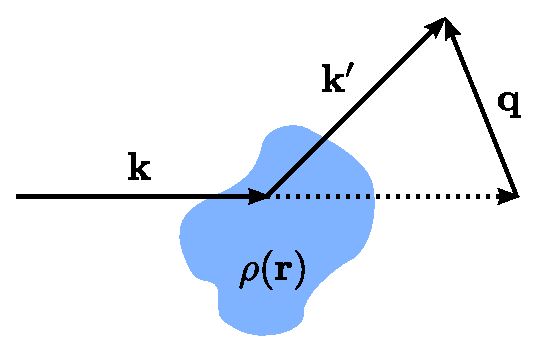
\includegraphics[width=0.5\textwidth]{diffraction/figures/scattering_vectors.eps}
\caption{Nomenclature of the scattering vectors. The incident wave is elastically scattered by a volume element $dV$ enclosing the charge $dQ = \rho(\mathbf{r}) dV$. The scattering vector $\mathbf{q}$ is the difference between the wavevectors $\mathbf{k}'$ and $\mathbf{k}$ and the scattered and the incident waves, respectively. The scattering angle, \emph{i.e.} the angle between $\mathbf{k}'$ and $\mathbf{k}$, is denoted by $2\theta$. \label{fig:elastic_scattering_vectors}}
\end{figure}

\noindent
Consider a charge density subject to a linearly polarized (classical) electromagnetic magnetic wave whose electric part is given by $\mathbf{E}_0 \cos (\mathbf{k}\cdot\mathbf{r}- \omega t)$. However, since the Maxwell equations and classical mechanics do not mix the real and imaginary parts, we may for mathematical convenience work with the complex exponential plane wave 
\begin{equation}\label{eq:complex_E_wave}
\mathbf{E}(\mathbf{r},t) = \mathbf{E}_0 e^{i \mathbf{k}\cdot\mathbf{r}-i \omega t},
\end{equation}
from which the physical field is recovered by taking its real part. Neglecting the effect of the magnetic field, the Lorentz force affecting an miniscule charge $dq$ in an infinitesimal volume element is
\begin{equation}
d\mathbf{F} = dq \ \mathbf{E}.
\end{equation}
Substituting the force from Newton's II law $\mathbf{F} = m \ddot{\mathbf{r}} \Rightarrow d\mathbf{F} = dm \ddot{\mathbf{r}}$, we obtain
\begin{equation}\label{eq:charge_acceleration}
\ddot{\mathbf{r}} = \frac{dq}{dm} \mathbf{E}.
\end{equation}
Since the nuclei of atoms are orders of magnitude more massive than electrons, we may ignore their movement and thus contribution to the scattering. Thus we can concentrate on the electronic contribution for which $dq/dm = -e/m$, where $e$ is the elementary charge and $m$ is the electron mass. Therefore by substituting the wavefield~\eqref{eq:complex_E_wave} to Eq.~\eqref{eq:charge_acceleration}, we get
\begin{equation}
\ddot{\mathbf{r}} = -\frac{e}{m} \mathbf{E}_0 e^{i \mathbf{k}\cdot\mathbf{r}-i \omega t}
\end{equation}
Integrating once with respect to time, we find that the velocity of an infititesimal charge $dq$ intially at rest is
\begin{equation}
\dot{\mathbf{r}} = -\frac{ie}{m\omega} \mathbf{E}_0 e^{i \mathbf{k}\cdot\mathbf{r}-i \omega t}.
\end{equation}
Therefore the current density $\mathbf{J}$ owing to oscillating electons becomes
\begin{equation}\label{eq:oscillating_J}
\mathbf{J}(\mathbf{r},t) = -en(\mathbf{r})\dot{\mathbf{r}} =
\frac{ie^2}{m\omega} n(\mathbf{r}) \mathbf{E}_0 e^{i \mathbf{k}\cdot\mathbf{r}-i \omega t}
\end{equation}
where $n(\mathbf{r})$ is the number density of electrons without the influence of external wavefield.

What kind of wavefield does the oscillating charge density emit? For that we need to solve the 
%wave equations for the scalar potential $\varphi$ and 
wave equation for the vector potential $\mathbf{A}$:
%\begin{align}
%\nabla^2 \varphi - \frac{1}{c^2}\frac{\partial^2 \varphi}{\partial t^2} &= -\frac{\rho}{\varepsilon_0} \\
%\nabla^2 \mathbf{A} - \frac{1}{c^2}\frac{\partial^2 \mathbf{A}}{\partial t^2} &= -\mu_0 \mathbf{J}
%\end{align}
\begin{equation}\label{eq:wave_function_A}
\nabla^2 \mathbf{A} - \frac{1}{c^2}\frac{\partial^2 \mathbf{A}}{\partial t^2} = -\mu_0 \mathbf{J}
\end{equation}
Since the $\nabla^2 - c^{-2} \partial^2_t$ is a linear operator, we seek the solution using the \emph{Green's function}. The Green's function $G(\mathbf{r},t;\mathbf{r}',t')$ is the solution to the problem 
\begin{equation}
\nabla^2  G(\mathbf{r},t;\mathbf{r}',t') - \frac{1}{c^2}\frac{\partial^2 G(\mathbf{r},t;\mathbf{r}',t')}{\partial t^2} = - \delta(\mathbf{r}-\mathbf{r}')
\delta(t-t').
\end{equation}
The solution to the inhomogeneous problem \eqref{eq:wave_function_A} is then
\begin{equation}
\mathbf{A}(\mathbf{r},t) = \mu_0 \int d\mathbf{r}' dt' \   \mathbf{J}(\mathbf{r}',t') G(\mathbf{r},t;\mathbf{r}',t').
\end{equation}
Since the retarded Green's function describing the solutions propagating away from the source is 
\begin{equation}
G(\mathbf{r},t;\mathbf{r}',t') = \frac{1}{4 \pi} \frac{\delta(t'-t_r)}{|\mathbf{r}-\mathbf{r}'|},
\end{equation}
where the retarded time $t_r = t - |\mathbf{r}-\mathbf{r}'|/c$ takes into account the finite speed of light, 
%the solutions to the wave equations are 
the formal solution to the wave equation is 
%\begin{align}
%\varphi &= \frac{1}{4 \pi \varepsilon_0}\int d\mathbf{r}' dt' \  \frac{\rho(\mathbf{r}',t')}{|\mathbf{r}-\mathbf{r}'|} \delta(t'-t_r) \\
%\mathbf{A} &= \frac{\mu_0}{4 \pi}\int d\mathbf{r}' dt' \  \frac{\mathbf{J}(\mathbf{r}',t')}{|\mathbf{r}-\mathbf{r}'|} \delta(t'-t_r).\label{eq:oscillating_A}
%\end{align}
\begin{equation}
\mathbf{A} = \frac{\mu_0}{4 \pi}\int d\mathbf{r}' dt' \  \frac{\mathbf{J}(\mathbf{r}',t')}{|\mathbf{r}-\mathbf{r}'|} \delta(t'-t_r).\label{eq:oscillating_A}
\end{equation}
%Since the atom is electrically neutral, the negative charge of the electron cloud is canceled by the positive nucleus. Sufficiently far away from the atom $\rho(\mathbf{r}',t')/|\mathbf{r}-\mathbf{r}'| \approx 0$, meaning that the scalar potential $\varphi$ vanishes. We are thus left only with a non-zero $\mathbf{A}$. 
Substituting $\mathbf{J}$ fom Eq.~\eqref{eq:oscillating_J} to Eq.~\eqref{eq:oscillating_A}, we get
\begin{align}
\mathbf{A} &= \frac{\mu_0}{4 \pi} \frac{ie^2}{m\omega} \mathbf{E}_0 \int d\mathbf{r}' dt' \  \frac{\delta(t'-t_r)}{|\mathbf{r}-\mathbf{r}'|} n(\mathbf{r}') e^{i \mathbf{k}\cdot\mathbf{r}'-i \omega t'} \nonumber \\ &= \frac{\mu_0}{4 \pi} \frac{ie^2}{m\omega} \mathbf{E}_0 \int d\mathbf{r}' \  \frac{n(\mathbf{r}')}{|\mathbf{r}-\mathbf{r}'|}  e^{i \mathbf{k}\cdot\mathbf{r}'-i \omega t_r}
\end{align}
Considering distances considerably larger than atomic dimensions, we may approximate $|\mathbf{r}-\mathbf{r}'|^{-1} \approx r^{-1}$. In addition, by substituting $t_r = t - |\mathbf{r}-\mathbf{r}'|/c$, we find
\begin{align}
\mathbf{A} &= \frac{\mu_0}{4 \pi} \frac{ie^2}{m\omega}\frac{1}{r} \mathbf{E}_0  \int d\mathbf{r}' \  n(\mathbf{r}')  e^{i \mathbf{k}\cdot\mathbf{r}'+i \omega |\mathbf{r}-\mathbf{r}'|/c -i \omega t} \nonumber \\ &= \frac{\mu_0}{4 \pi} \frac{ie^2}{m\omega}\frac{1}{r} \mathbf{E}_0  e^{-i \omega t} \int d\mathbf{r}' \  n(\mathbf{r}')  e^{i \mathbf{k}\cdot\mathbf{r}'+i k |\mathbf{r}-\mathbf{r}'|},
\end{align}
where in the last step $k=\omega/c$ has been used. By denoting the outgoing wavevector by $\mathbf{k}'$, we recognize that
\begin{equation}
k|\mathbf{r}-\mathbf{r}'| = \mathbf{k}'\cdot(\mathbf{r}-\mathbf{r}') 
\end{equation}
In principle, the direction of $\mathbf{k}'$ depends on $\mathbf{r}'$ but far away from the atom we can regard it being constant. Thus
\begin{equation}
\mathbf{A} = \frac{\mu_0}{4 \pi} \frac{ie^2}{m\omega}\frac{1}{r} \mathbf{E}_0  e^{i \mathbf{k}'\cdot\mathbf{r}-i \omega t} \int d\mathbf{r}' \  n(\mathbf{r}')  e^{i (\mathbf{k}-\mathbf{k}')\cdot\mathbf{r}'}.
\end{equation}

Since we haven't calculated the scalar potential $\varphi$, we can't directly obtain the electric field $\mathbf{E} = -\nabla \varphi - \partial \mathbf{A}/ \partial t$ from the potential.  Therefore we first compute the magnetic field
\begin{equation}
\mathbf{B}' = \nabla \times \mathbf{A} = -\frac{\mu_0}{4 \pi} \frac{e^2}{m\omega}\frac{1}{r} \mathbf{k}' \times \mathbf{E}_0  e^{i \mathbf{k}'\cdot\mathbf{r}-i \omega t} \int d\mathbf{r}' \  n(\mathbf{r}')  e^{i (\mathbf{k}-\mathbf{k}')\cdot\mathbf{r}'},
\end{equation}
where we have benefited from the fact that $e^{i \mathbf{k}'\cdot\mathbf{r}}$ varies considerably faster than $r^{-1}$, thus dominating the derivative. The electric field is now found using the Maxwell's equations. Assuming the plane wave form $\mathbf{E}' e^{i \mathbf{k}'\cdot\mathbf{r}-i \omega t}$, the time derivative of the field is
\begin{equation}
\frac{\partial}{\partial t} \mathbf{E}' e^{i \mathbf{k}'\cdot\mathbf{r}-i \omega t}
= -i \omega \mathbf{E}' e^{i \mathbf{k}'\cdot\mathbf{r}-i \omega t}.
\end{equation}
In the absence of free currents, $\partial \mathbf{E}' /\partial t = c^2 \nabla \times \mathbf{B}'$. Therefore for the plane waves in question $\mathbf{E}' = -c^2/\omega \mathbf{k}' \times \mathbf{B}'$. Thus
\begin{equation}
\mathbf{E}' = \frac{1}{4 \pi \varepsilon_0} \frac{e^2}{mc^2}\frac{1}{r} \frac{\mathbf{k}' \times(\mathbf{k}' \times \mathbf{E}_0)}{k^2}  e^{i \mathbf{k}'\cdot\mathbf{r}-i \omega t} \int d\mathbf{r}' \  n(\mathbf{r}')  e^{i (\mathbf{k}-\mathbf{k}')\cdot\mathbf{r}'},
\end{equation}
where $c^2 = 1/\epsilon_0 \mu_0$ has been used. 
The quantity we measure in the scattering experiments is not the electric field, however, but the time-averaged intensity of the field. Since the intensity is proportional to $|\mathbf{E}|^2$, the ratio of the scattered intensity $I$' to the incident intensity $I$ is  
\begin{equation}
\frac{I'}{I} =  \frac{|\mathbf{E}'|^2}{|\mathbf{E}|^2}
\end{equation}
Since 
\begin{align}
\mathbf{k}' \times(\mathbf{k}' \times \mathbf{E}_0) &= (\mathbf{k}'\cdot \mathbf{E}_0)\mathbf{k}' - k^2 \mathbf{E}_0 = k |\mathbf{E}_0| \cos \chi \mathbf{k}'  - k^2 \mathbf{E}_0 \nonumber \\ \Rightarrow
|\mathbf{k}' \times(\mathbf{k}' \times \mathbf{E}_0)|^2 &=
k^2 |\mathbf{E}_0|^2 \cos^2 \chi \mathbf{k}' \cdot \mathbf{k}'
-2 k^3 |\mathbf{E}_0| \cos \chi \mathbf{k}'\cdot \mathbf{E}_0 + k^4 |\mathbf{E}_0|^2 \nonumber \\
&= (1 - \cos^2 \chi) k^4 |\mathbf{E}_0|^2 = \sin^2 \chi k^4 |\mathbf{E}_0|^2,
\end{align}
where $\chi$ is the angle between the polarization of the incident wave and the scattering vector, we obtain
\begin{equation}
\frac{I'}{I} = \left(\frac{e^2}{4\pi\varepsilon_0 m c^2} \right)^2 \frac{1}{r^2} \sin^2 \chi \left|\int d\mathbf{r}' \  n(\mathbf{r}')  e^{i (\mathbf{k}-\mathbf{k}')\cdot\mathbf{r}'} \right|^2.
\end{equation}
The expression of intensity ratio still contains the factor of $r^{-2}$ which is basically a parameter depending on the experiment setup, not the system itself. In scattering studies, it is customary to use the so-called \emph{differential scattering cross section} $d \sigma / d\Omega$ as the 
quantity of interest instead. By definition $d \sigma / d\Omega$ is the fraction of intensity (or particles) scattered into a given direction. Since the infinitesimal area $dA = r^2 d \Omega$, where $d \Omega$ is the solid angle corresponding to the area, we find that the differential cross-section is
\begin{equation}
\frac{d \sigma}{d \Omega} = \left(\frac{e^2}{4\pi\varepsilon_0 m c^2} \right)^2 \sin^2 \chi \left|\int d\mathbf{r}' \  n(\mathbf{r}')  e^{-i \mathbf{q}\cdot\mathbf{r}'} \right|^2.
\end{equation}
where the \emph{scattering vector} $\mathbf{q} = \mathbf{k}' - \mathbf{k}$. 

The derived cross section consists of two factors. The first one is the well-known \emph{Thomson differential cross section}
\begin{equation}
\left(\frac{d \sigma}{d \Omega}\right)_{\rm Th} = \left(\frac{e^2}{4\pi\varepsilon_0 m c^2} \right)^2 \sin^2 \chi,
\end{equation}
which describes the scattering by a free electron. Quite often the Thomson differential cross-section is seen given for the unpolarized radiation, when it obtains the form
\begin{equation}
\left(\frac{d \sigma}{d \Omega}\right)_{\rm Th} = \left(\frac{e^2}{4\pi\varepsilon_0 m c^2} \right)^2 \frac{1+\cos^2 2 \theta}{2},
\end{equation}
where $2\theta$ is the scattering angle.

The structure of the electron density, on the other hand, is totally contained in the second factor. We may recognize the integral as the Fourier transform of the charge density. Thus by measuring the elastic differential scattering cross section as the function of $\mathbf{q}$, we can obtain direct information about the distribution of the charge density. However, we can not obtain the full $n(\mathbf{r})$ through inversion, since we can measure only the amplitude of the Fourier transform and not its phase. For example consider a large number of identical particles which are distributed randomly at positions $\mathbf{r}_i$. If the electron density of a single particle is described by $\eta(\mathbf{r}-\mathbf{r}_i)$, then its Fourier transform is
\begin{equation}
\int d\mathbf{r}' \  \eta(\mathbf{r}'-\mathbf{r}_i)  e^{-i \mathbf{q}\cdot\mathbf{r}'} = \int d\mathbf{r}' \ \eta(\mathbf{r}')  e^{-i \mathbf{q}\cdot(\mathbf{r}'+\mathbf{r}_i)} = 
e^{-i \mathbf{q}\cdot\mathbf{r}_i}
\int d\mathbf{r}' \  \eta(\mathbf{r}')  e^{-i \mathbf{q}\cdot\mathbf{r}'},
\end{equation}
\emph{i.e.} the Fourier transforms of the particles differ only by the phase factor $e^{-i \mathbf{q}\cdot\mathbf{r}_i}$. This information is lost in the scattering, so we can't say anything about the positions of the individual particles but we can say obtain some knowledge about the electron density $\eta(\mathbf{r})$. Nevertheless, a lot of information on $\eta(\mathbf{r})$ is lost as well, especially if the particles are highly asymmetric. However, as we well see in the following sections, some of the phase information can be retained if the particles are organised in a periodic manner.